\chapter{Úvod}
\label{kap:uvod}
Česká republika patří mezi země s~nejhustší sítí železnic na světě. Každým rokem se pro všechny tratě v~této síti vytváří plán jízdy vlaků, zohledňující velké množství často protichůdných požadavků. Cestující se s~částmi tohoto plánu, jízdami vlaků určených pro osobní dopravu, seznamují skrze tištěné knižní jízdní řády nebo uživatelsky přívětivé webové služby. Před běžnými cestujícími tak zůstává skryté množství pomůcek určených pro služební účely. Jednou z~takových pomůcek je nákresný jízdní řád, jehož příklad můžeme vidět na obrázku \ref{fig:uvod:njr_bez_anotaci}.

\begin{figure}[ht]
	\centering
	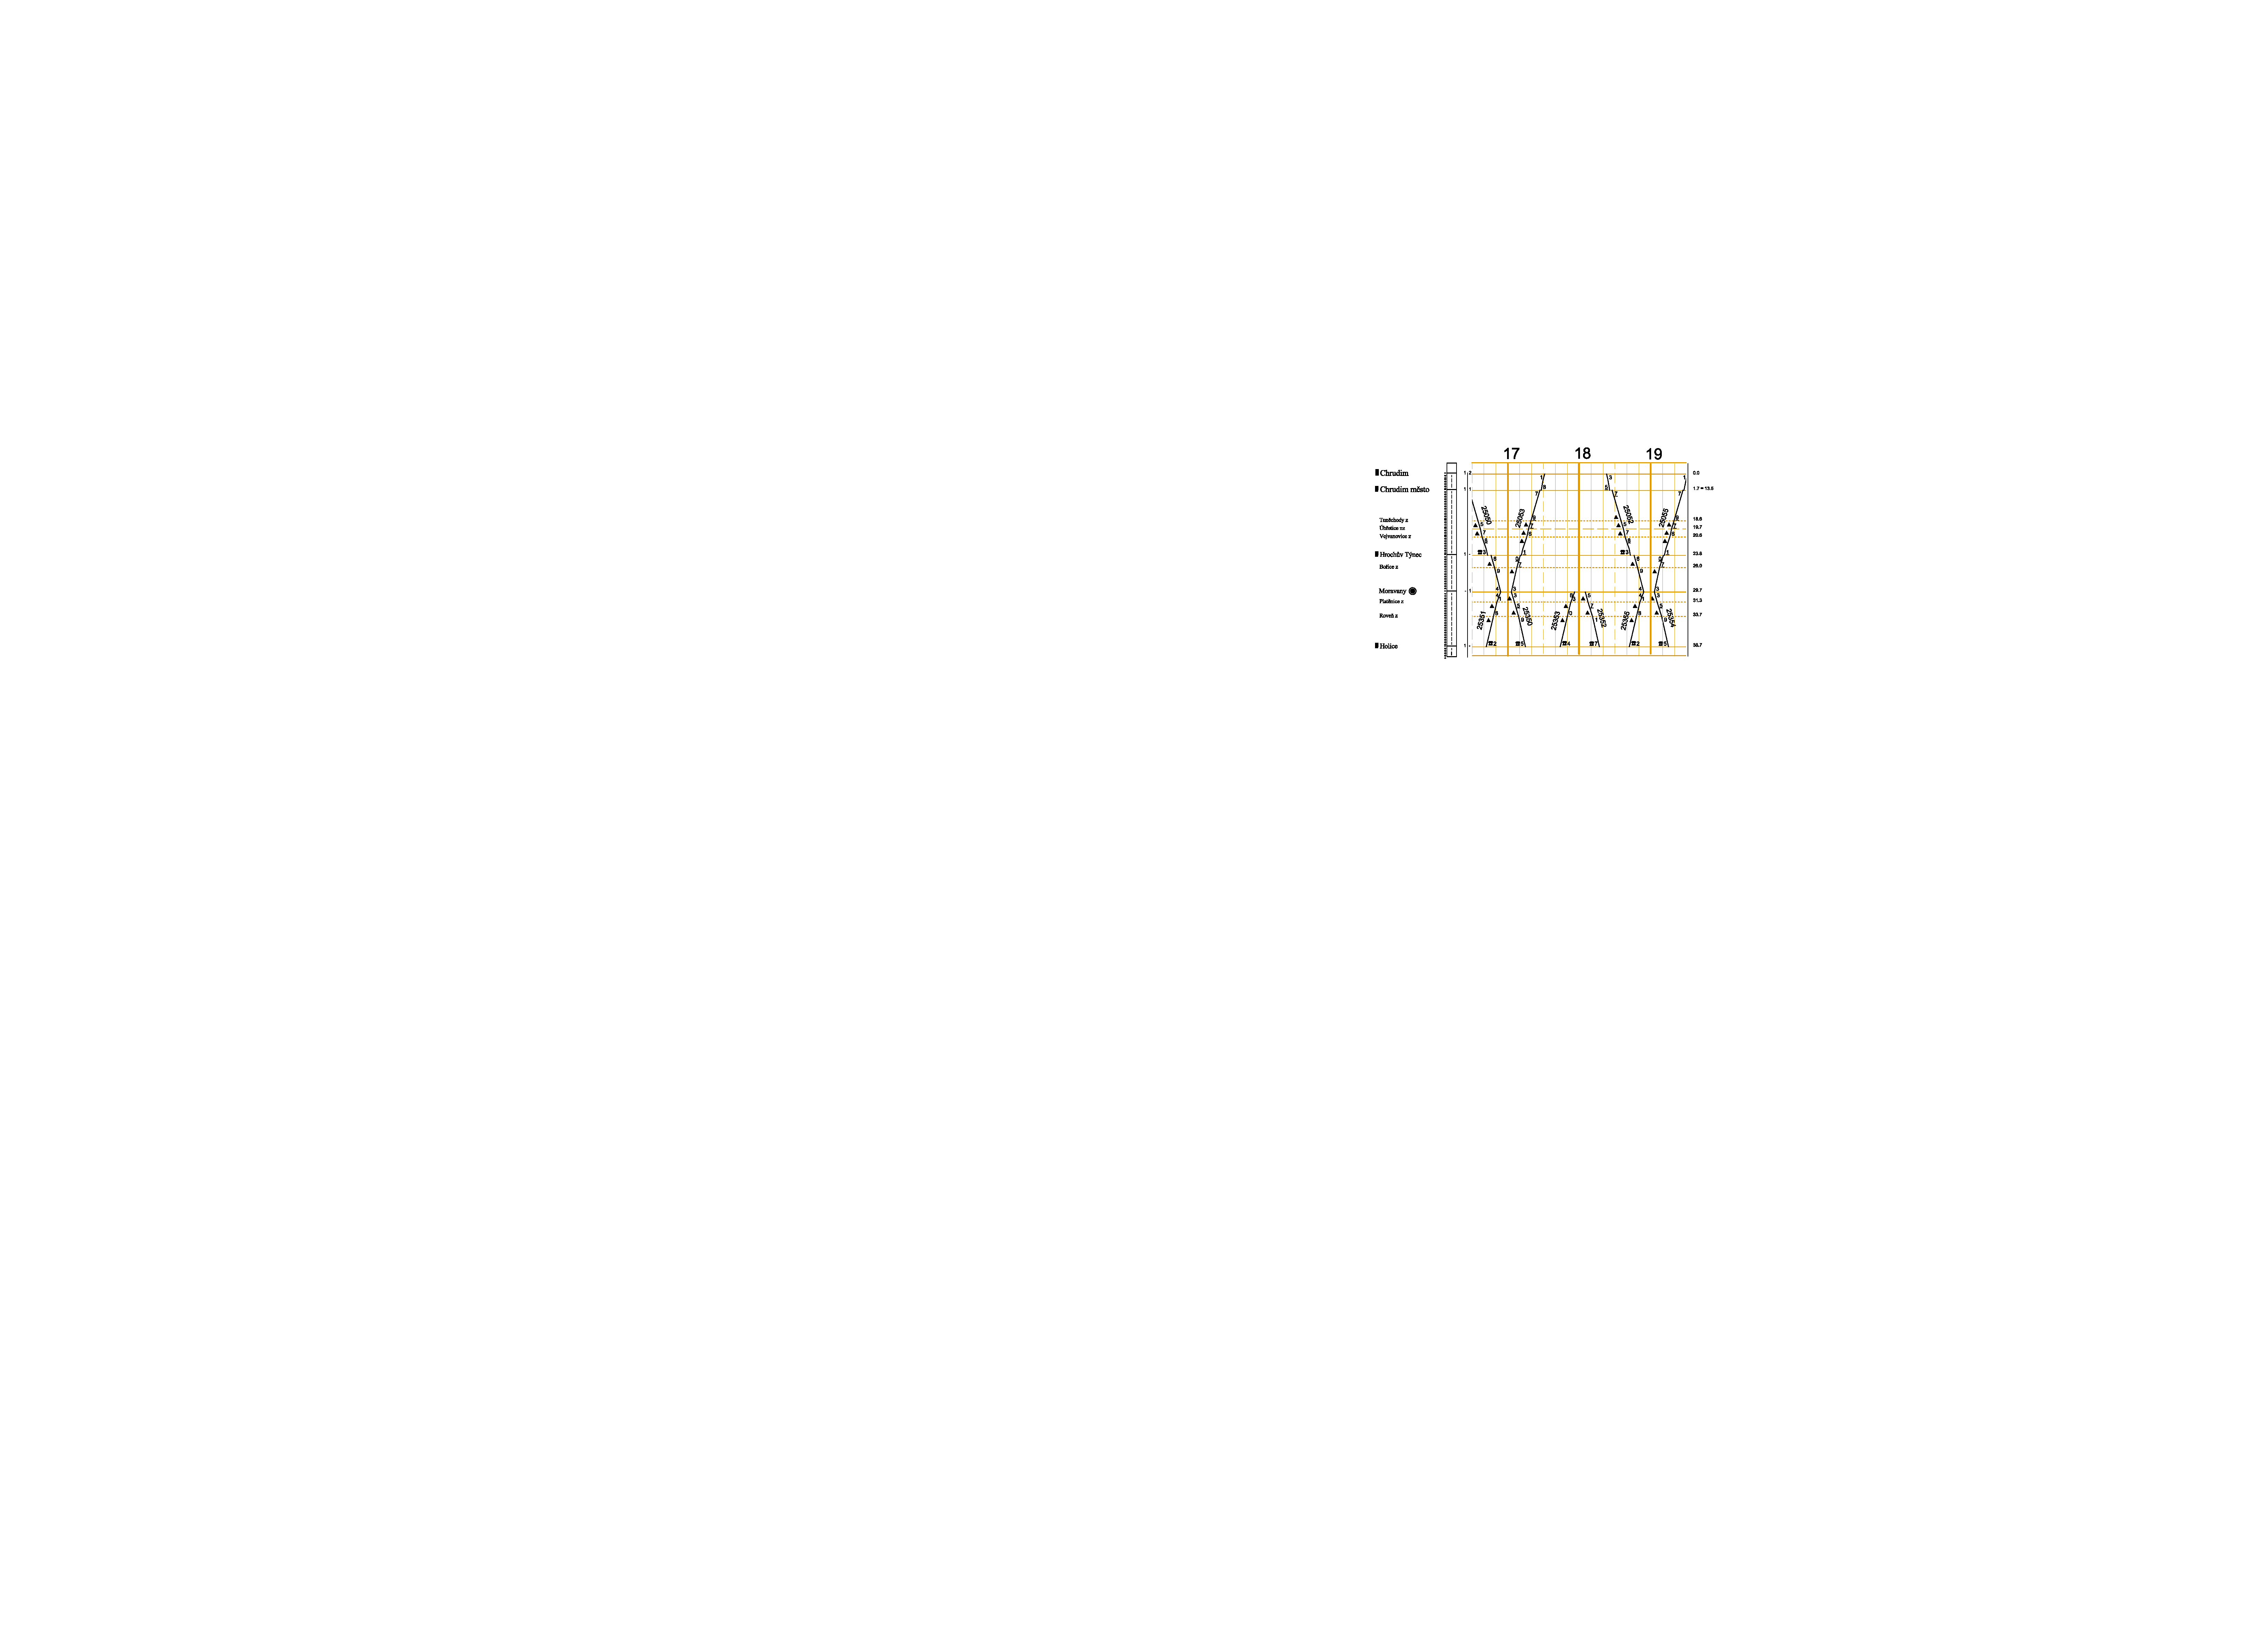
\includegraphics[width=\textwidth]{../img/kap1_uvod_grafikon}
	\caption{Příklad nákresného jízdního řádu}
	\label{fig:uvod:njr_bez_anotaci}
\end{figure}

Všichni zaměstnanci zúčastněni na provozu železniční dopravy potřebují mít přehled o~plánovaném i~aktuálním provozu v~traťových úsecích. Jelikož pro tuto potřebu reprezentovat data textovou formou není vhodné, využívá se znázornění průběhu jízd vlaků ve formátu, který se v~železniční dopravě označuje jako \textit{nákresný jízdní řád}. 
Existují aplikace, které s~nákresným jízdním řádem pracují. Aplikace se však často při jeho zobrazování potýkají s~problémy. Dále existují nástroje, které ke svému fungování nákresný jízdní řád nepotřebují, ale práce s~nimi by se mohla zlepšit, pokud budou nákresný jízdní řád zobrazovat. Chtěli bychom proto vytvořit nástroj, který bude nákresné jízdní řády zobrazovat a~umožní s~nimi co nejlépe pracovat. Hlavním cílem práce bude vytvořit takový nástroj jako grafickou komponentu integrovatelnou do různých aplikací.

Než ale blíže určíme, jaké konkrétní požadavky by měla tato grafická komponenta splňovat, podrobně si v~této kapitole nákresný jízdní řád představíme a~zvážíme jeho existující uplatnění i~možná využití. Jeho vlastnosti, které si budeme popisovat, jsou často specifické pro české prostředí.

\section{Nákresné jízdní řády}
\label{kap:uvod:nakresny_jizdni_rad}

Základem nákresného jízdního řádu je síť vodorovných a~svislých čar umístěná v~grafu, který je znázorněn na obrázku \ref{fig:uvod:njr_graf}. Svislou osou grafu je kilometrická poloha na trati. Vodorovná osa značí čas, kde čísla na obrázku představují celé hodiny.

\begin{figure}[ht]
	\centering
	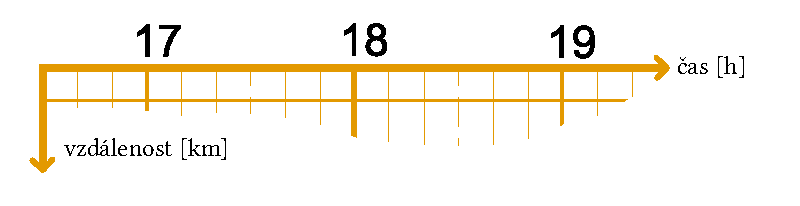
\includegraphics[width=0.7\textwidth]{../img/kap1_njr_graf}
	\caption{Osy nákresného jízdního řádu}
	\label{fig:uvod:njr_graf}
\end{figure}

Význam vodorovných a~svislých čar si vysvětlíme s~pomocí obrázku \ref{fig:uvod:njr_osy}, který obsahuje nákresný jízdní řád doplněný anotacemi ke zmíněným čarám.

Na trati se nachází významná místa (například stanice, zastávky nebo výhybny), které označujeme jako \textit{dopravní body}. Vodorovné čáry odpovídají dopravním bodům rozmístěných v~grafu podle jejich kilometrické polohy vzhledem k~trati. Na obrázku \ref{fig:uvod:njr_osy} pro přehlednost modře podbarvená plná čára reprezentuje stanici Chrudim. Přerušovaná čára podbarvená zelenou barvou patří nákladišti a~zastávce Úhřetice. Červeně podbarvená tečkovaná čára značí zastávku Bořetice. Vzor (nebo i~tloušťka) čáry tak určuje typ dopravního bodu.

Stejným způsobem se rozlišují svislé čáry značící časové údaje v~intervalech po deseti minutách. Plná čára na obrázku \ref{fig:uvod:njr_osy} označena 
\includegraphics[height=10.0pt]{../img/cas_osa_typ_1} je určena pro hodiny, 
\includegraphics[height=10.0pt]{../img/cas_osa_typ_2} pro půlhodiny a~tenká plná čára označená 
\includegraphics[height=10.0pt]{../img/cas_osa_typ_3} je určena pro jiné časové údaje.

\begin{figure}[ht]
	\centering
	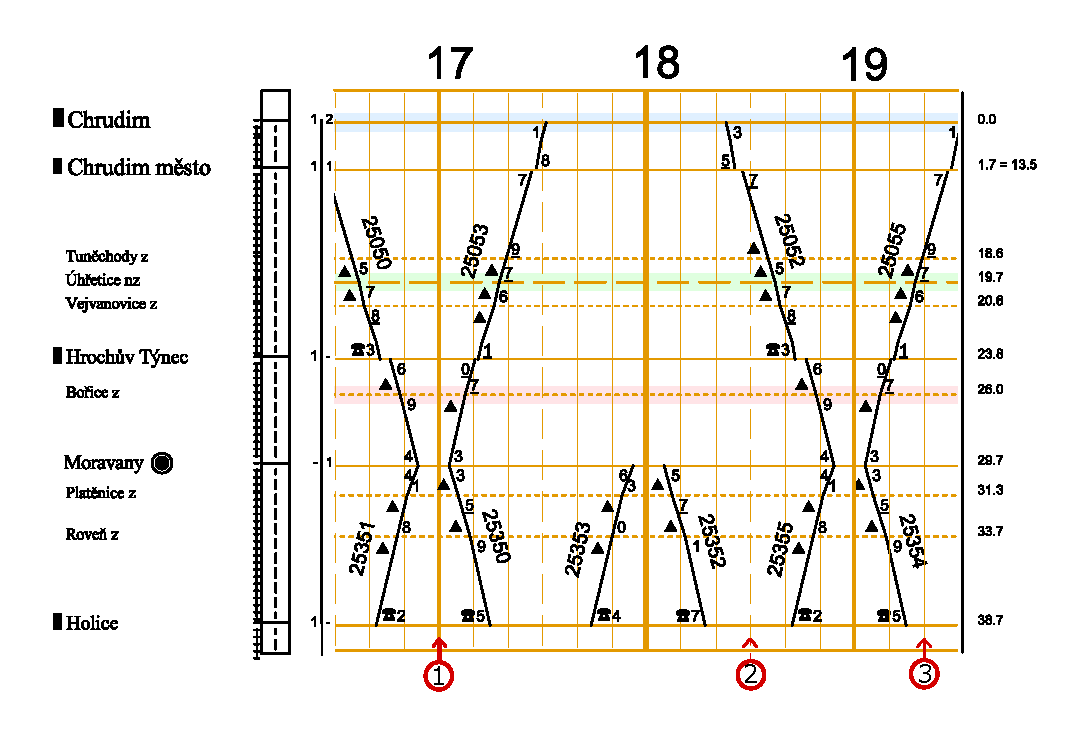
\includegraphics[width=\textwidth]{../img/kap1_uvod_grafikon_osy}
	\caption{Nákresný jízdní řád s~vyznačenými typy vodorovných a~svislých čar}
	\label{fig:uvod:njr_osy}
\end{figure}

\subsection*{Průběh jízdy vlaků v~nakresném jízdním řádu}
Popsaná síť vodorovných a~svislých čar je nutným základem pro vyobrazení nejdůležitějšího obsahu nákresného jízdního řádu, kterým jsou průběhy jízd vlaků. Pomocí obrázku \ref{fig:uvod:njr_vlaky} obsahující zvýrazněné průběhy jízd některých vlaků si popíšeme princip jejich vyobrazování.

\begin{figure}[ht]
	\centering
	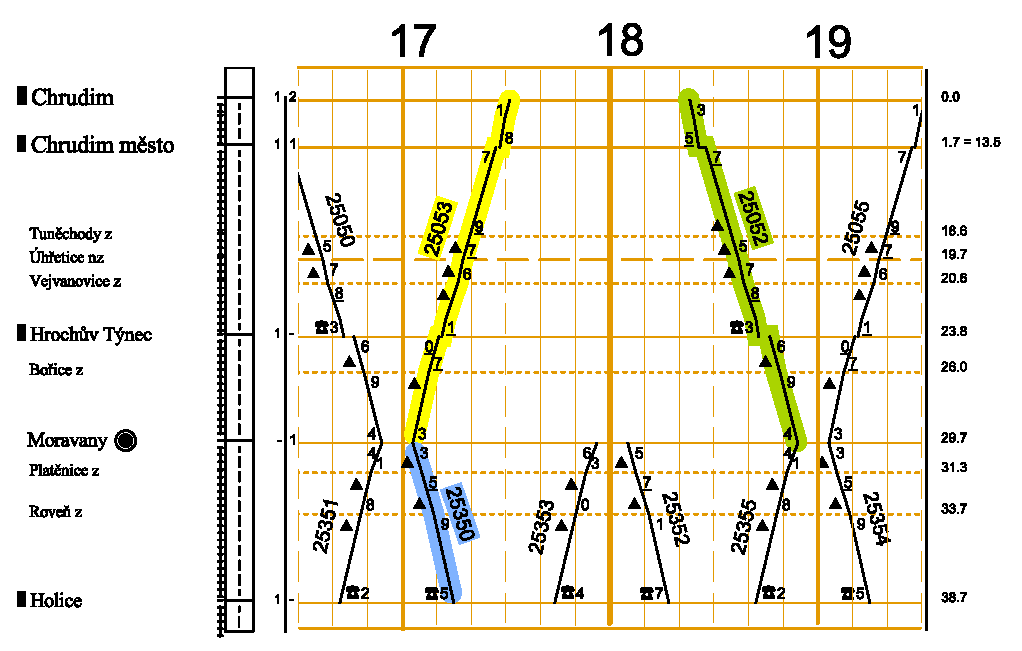
\includegraphics[width=\textwidth]{../img/kap1_uvod_grafikon_vlaky}
	\caption{Nákresný jízdní řád s~vyznačenými průběhy jízd vlaků 25350, 25052 a~25053}
	\label{fig:uvod:njr_vlaky}
\end{figure}

Na obrázku \ref{fig:uvod:njr_vlaky} se nachází vlak označený číslem 25053 se žlutě podbarvenou šikmou čarou reprezentující průběh jeho jízdy. Všimněme si, že tato čára tvoří průsečíky s~vodorovnými čarami reprezentující dopravní body. Takový průsečík pak představuje příjezd, odjezd nebo průjezd vlaku dopravním bodem v~čase, který odpovídá pozici průsečíku na časové ose. Průsečík šikmé čáry, který se vyskytne na časové ose jako první, patří k~dopravnímu bodu, ze kterého vlak vyjíždí. Poslední průsečík naopak odpovídá dopravnímu bodu, kde jízda vlaku končí. V~případě vlaku 25053 vlak vyjíždí přibližně v~sedmnáct hodin ze stanice Moravany a~jede směrem na Chrudim, do které dojede kolem půl šesté. Tímto popsaným principem můžeme sledovat celý průjezd vlaku tratí v~závislosti na čase a~jeho poloze.

Podobně je možné z~obrázku \ref{fig:uvod:njr_vlaky} určit průběh jízdy i~u~ostatních vlaků. Zeleně podbarvená lomená čára představuje průběh jízdy vlaku 25052, který jede v~opačném směru do Moravan. Modře podbarvený vlak 25350 odjíždí z~Moravan ve stejný čas jako vlak 25053, ale v~opačném směru na Holice. Svislé čáry těchto dvou vlaků, které jsou vizuálně spojeny v~Moravanech, od sebe můžeme odlišit pochopením faktu, že kdybychom je vnímaly jako celek zobrazující průběh jízdy jednoho vlaku, záznam by vzhledem k~časové ose nedával smysl, jelikož by se vracel do minulosti.

\pagebreak

Nezbytnou součástí vyobrazení informací o~jízdě vlaků v~nákresném jízdním řádu je vhodně umístěné číslo vlaku v~blízkosti šikmé čáry, která odpovídá průběhu jeho jízdy. Podle pravidel provozu na českých železničních tratích má každý vlak přiděleno unikátní číslo. Číslo je v~nákresném jízdním řádu umístěno způsobem, z~kterého je zřejmé, k~jakému vlaku patří. Číslo se umisťuje v~blízkosti šikmé čáry vlaku tak, aby směr čtení čísla odpovídal směru jízdy. Šikmá čára je pak pomyslným řádkem, na kterém je číslo napsáno.

\subsubsection*{Výhody zobrazování průběhu jízd vlaků nákresným jízdním řádem}

Abychom pochopili, v~jakých situacích je možné nákresné jízdní řády používat, popíšeme si výhody, které přináší oproti jiným formám jízdního řádu. Z~nákresného jízdního řádu je lehké zjistit, jak jsou úseky mezi dopravními body obsazeny jízdami vlaků. Drážní zaměstnanec tak má přehled o~dopravní situaci na celé trati.

Vedle nákresných jízdních řádů existují jízdní řády v~textové formě, které jsou užitečné například pro cestující, ale nemůžou nahradit roli nákresného jízdního řádu. Jedním z~textových formátů zobrazující informace o~jízdě vlaků je knižní jízdní řád, jehož výřez je uvedený na obrázku \ref{fig:uvod:kjr}. Můžeme vidět, že informace v~něm obsažené jsou vztaženy k~jen konkrétnímu vlaku a~těžko se mezi sloupečky, obsahující plány jízd vlaků, dají hledat hlubší souvislosti. Pro porovnání jsou vlaky z~výřezu knižního jízdního řádu vyobrazeny na nákresném jízdním řádu na obrázku \ref{fig:uvod:njr_vyrez}.

\begin{figure}[ht]
	\centering
	\includegraphics[width=\textwidth]{../img/kap1_uvod_grafikon_kjr_vyrez}
	\caption{Nákresný jízdní řád s~podbarvenými průběhy jízd vlaků z~knižního jízdního řádu na obrázku \ref{fig:uvod:kjr}}
	\label{fig:uvod:njr_vyrez}
\end{figure}

\begin{figure}[ht]
	\centering
	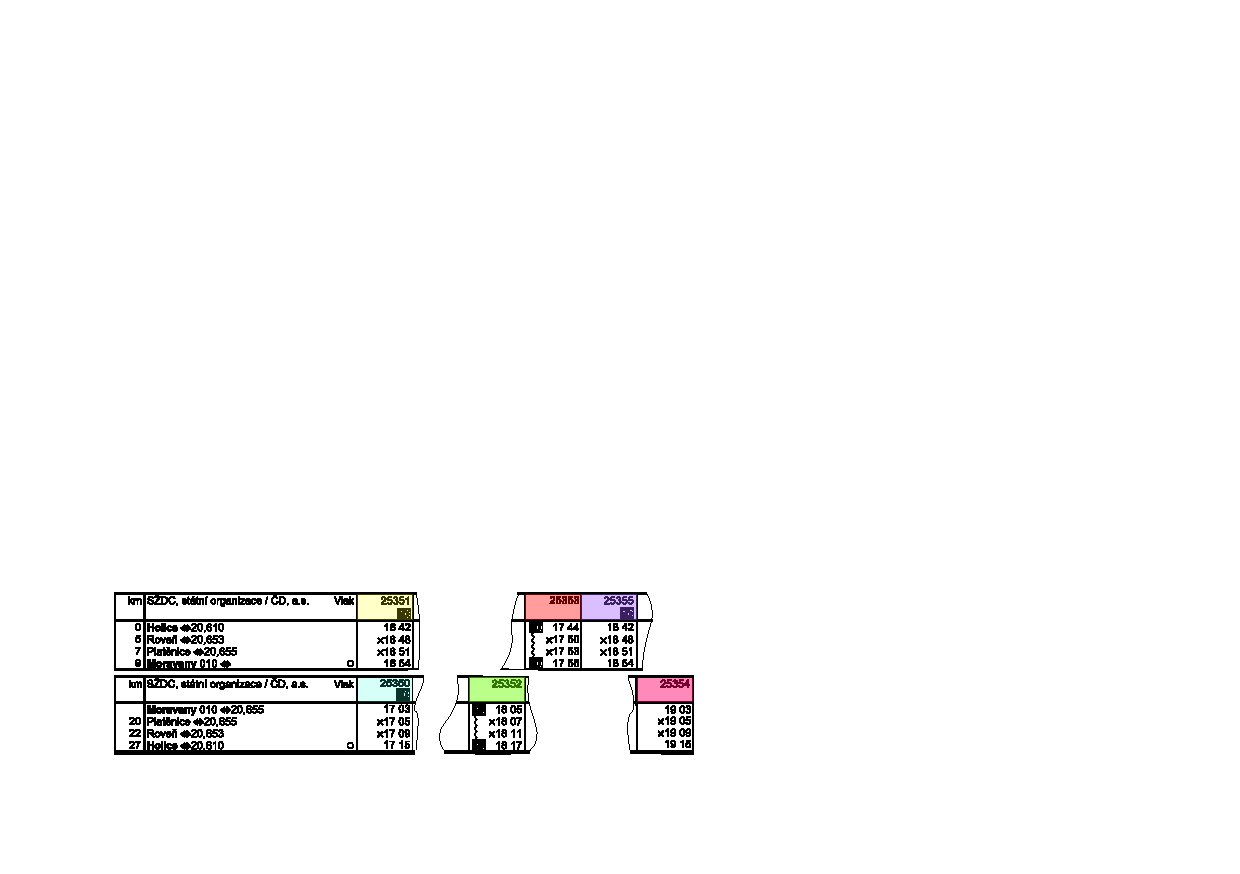
\includegraphics[width=0.9\textwidth]{../img/kap1_kjr_moravany_holice_vyrez}
	\caption{Výřez z~knižního jízdního řádu se zvýrazněnými čísly vlaků odpovídající podbarveným průběhům jízd těchto vlaků na obrázku \ref{fig:uvod:njr_vyrez}}
	\label{fig:uvod:kjr}
\end{figure}

V~další části si popíšeme, jak z~nákresného jízdního řádu můžeme vyčíst přesné časy příjezdů a~odjezdů obsažených ve sloupcích knižních jízdních řádů.

\subsection*{Informace k~jízdě vlaků v~nákresném jízdním řádu}
\label{kap1:koty_a_informace_o_prubehu_vlaku}
Ještě jsme si neuvedli, jak v~nákresných jízdních řádech určit přesný čas příjezdů, odjezdů a~průjezdů vlaku dopravními body. Tyto informace se nachází v~ostrých úhlech, které dopravní body s~trasami vlaků svírají, a~nazývají se \textit{kóty}. V~kótách se pouze uvádí jednotky minut, například pro čas 19:15 se uvede 5. Na obrázku \ref{fig:uvod:koty} můžeme vidět, jak jsou tímto způsobem ve výřezu nákresného jízdního řádu zaznamenány časy odjezdů (a~příjezdu do Holic) z~knižního jízdního řádu.

\begin{figure}[ht]
	\centering
	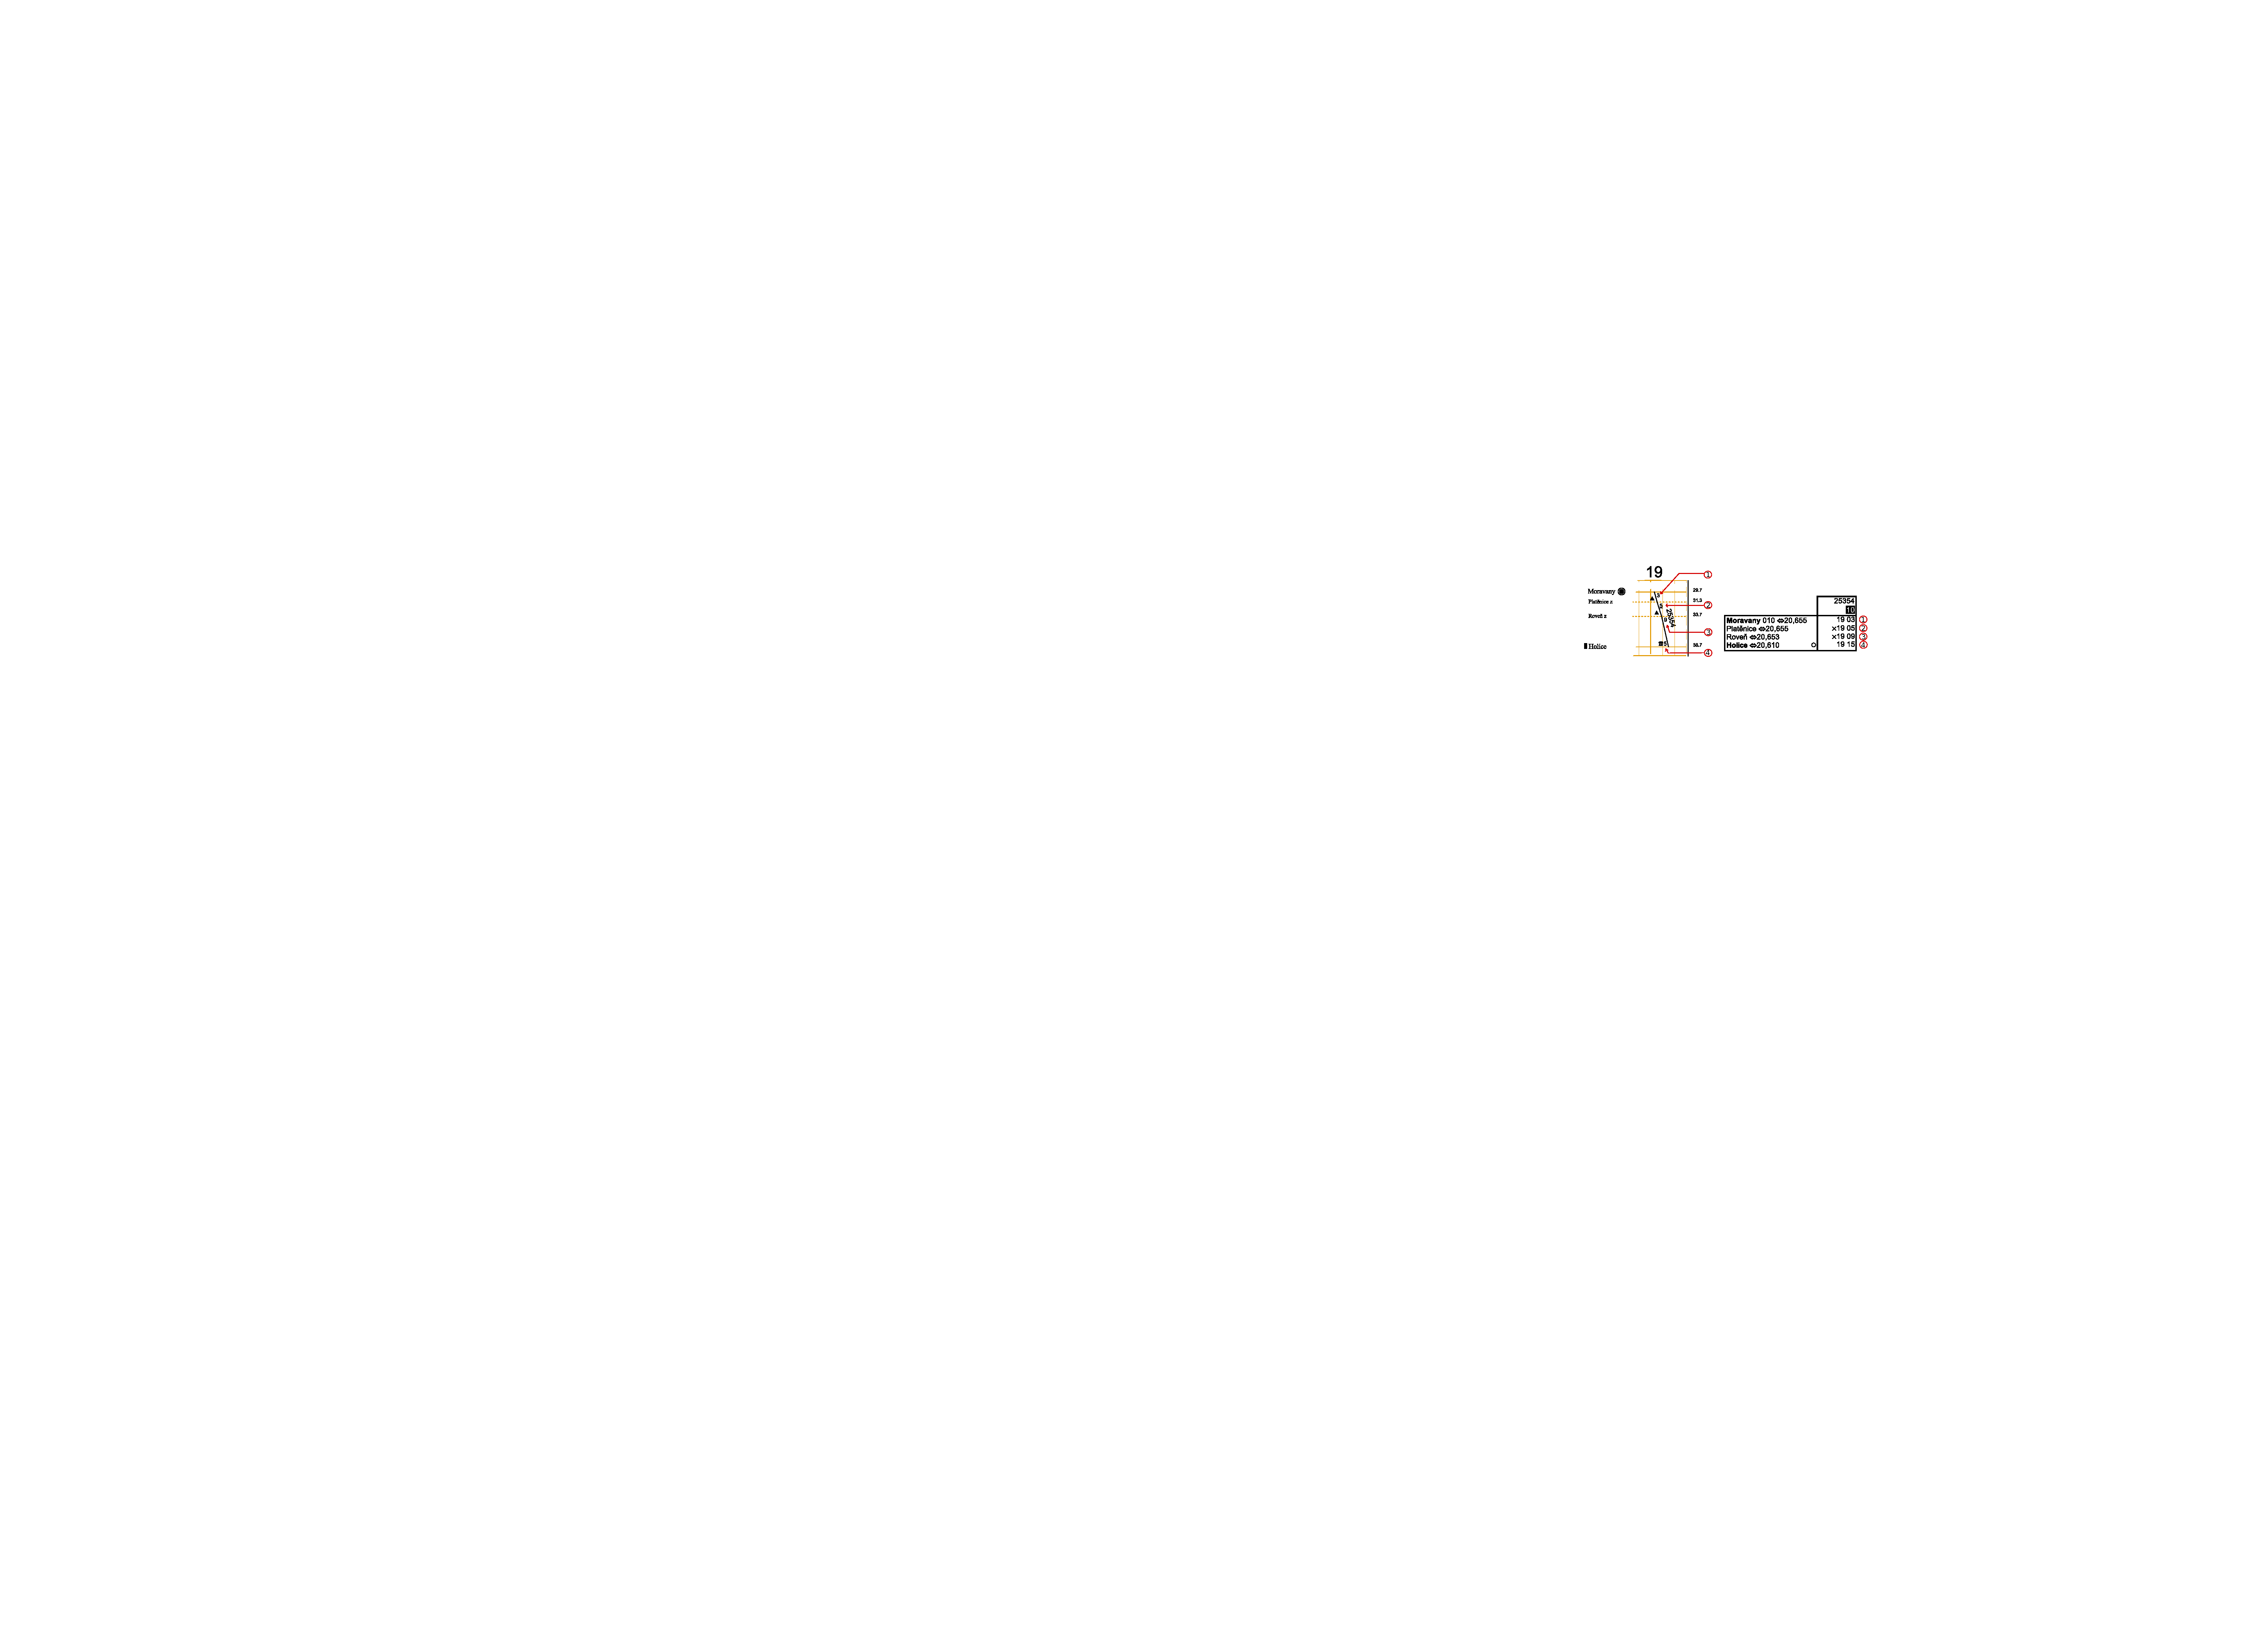
\includegraphics[width=\textwidth]{../img/kap1_koty_popis}
	\caption{Označené kóty v~nákresném jízdním řádu odpovídající časům v~knižním jízdním řádu}
	\label{fig:uvod:koty}
\end{figure}

Ostré úhly neslouží pouze k~umisťování kót, ale je možné do nich přidat i~další informace, které by se musely jinak složitě hledat jinde. Navíc se někdy zobrazení kót mění. Příklady zmiňovaných informací a~změn se nachází na obrázku \ref{fig:uvod:koty_dalsi}:

\begin{enumerate}[label=(\alph*)]
\item Ikona telefonu značí ohlašovací povinnost strojvedoucího při příjezdu do dopravního bodu.
\item Pokud má vlak v~dopravním bodu dobu pobytu kratší než půl minuty a~nejedná se o~průjezd, kóta příjezdu se nahradí trojúhelníkem.
\item Podtržená kóta značí o~půlminuty více. Na obrázku vlak odjíždí z~dopravního bodu mezi pěti minutami a~30 sekundami až šesti minutami, vhledem k~používanému zaokrouhlení času pro kóty.
\end{enumerate}

\begin{figure}[ht]
    \centering
    \begin{subfigure}[b]{0.3\textwidth}
        
\includegraphics[width=0.7\textwidth]{../img/koty_dalsi_set_x}
        \caption{Ohlašovací povinnost nařízena}
    \end{subfigure}
    \begin{subfigure}[b]{0.3\textwidth}
        
\includegraphics[width=0.7\textwidth]{../img/koty_dalsi_set_y}
        \caption{Pobyt kratší než půl minuty}
    \end{subfigure}
    \begin{subfigure}[b]{0.3\textwidth}
        
\includegraphics[width=0.7\textwidth]{../img/koty_dalsi_set_z}
        \caption{Odjezd o~půl minuty později}
    \end{subfigure}
    \caption{Další informace umístitelné do ostrých úhlů}
    \label{fig:uvod:koty_dalsi}    
\end{figure}

\newpage
\subsection*{Další informace zobrazované v~nákresných jízdních řádech}
\label{kap1:dalsi_info}
Doposud jsme si popisovali, jak se zobrazují informace související s~jízdou vlaku. Nákresný jízdní řád se ale nemusí omezovat pouze na tyto informace. Na obrázku \ref{fig:uvod:njr_doplnky} můžeme vidět několik sloupců. Zeleně podbarvený sloupec obsahuje názvy dopravních bodů, umístěných podle kilometrické vzdálenosti na trati. V~blízkosti názvů se pak nachází značení, přidávající další informace o~dopravním bodu. Ve fialově podbarveném sloupci se nachází informace o~zabezpečení traťového úseku. Oranžově podbarvený sloupec zobrazuje kilometrické vzdálenosti dopravních bodů na trati.

\begin{figure}[ht]
	\centering
	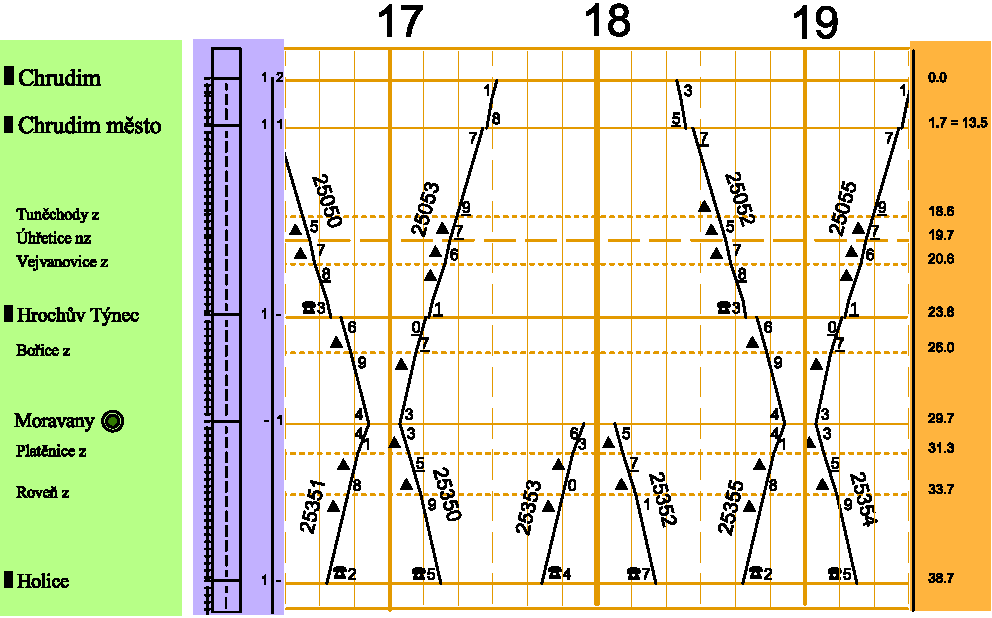
\includegraphics[width=0.85\textwidth]{../img/kap1_uvod_grafikon_doplnky}
	\caption{Nákresný jízdní řád s~podbarvenými sloupci nesoucí další informace}
	\label{fig:uvod:njr_doplnky}
\end{figure}

Tímto jsme dokončili popis všech informací v~nákresném jízdním řádu, poprvé uvedeném na obrázku \ref{fig:uvod:njr_bez_anotaci}.

\subsection*{Další typy nákresných jízdních řádů}
Až do této chvíle jsme si pro lehčí pochopení ukazovali pouze jeden typ nákresného jízdního řádu. Existuje ale více typů nákresných jízdních řádů. Nákresný jízdní řád na obrázku \ref{fig:uvod:slovensky_njr} se používá pro organizaci železniční dopravy na Slovensku a~jeho vizualizace se řídí doposud uvedenými pravidly, pouze se liší v~drobnostech, kterými jsou použité barvy nebo vzor čar.

\begin{figure}[ht]
	\centering
	
\includegraphics[width=\textwidth]{../img/kap1_slovensko}
	\caption{Další typ nákresného jízdního řádu}
	\label{fig:uvod:slovensky_njr}
\end{figure}
\newpage
Než si ale detailně uvedeme jiné typy nákresných jízdních řádů, které budou obvykle součástí různých aplikací, zasadíme je do kontextu grafikonu vlakové dopravy, s~kterým tyto aplikace pracují.

\section{Grafikon vlakové dopravy}
V~železniční dopravě se pracuje s~pojmem grafikon vlakové dopravy. Ten je v~přeneseném významu jiným označením pro zobrazení jízdy vlaků v~nákresném jízdním řádu. Proto se někdy nákresné jízdní řády označují jako listy grafikonu vlakové dopravy. Původně ale tento pojem představuje označení pro soubor předpisů a~pomůcek určených k~plánování vlakové dopravy. Na základě mnoha často protichůdných požadavků se pomocí předpisů a~pravidel grafikonu vlakové dopravy sestaví plán, sloužící jako předloha a~dokumentace, na kterou je se potřeba při organizaci dopravy a~řešení konfliktů vznikajících při provozu odkazovat. Takto sestavený plán je obsažen v~pomůckách grafikonu vlakové dopravy, mezi které patří právě listy nákresného jízdního řádu nebo jízdní řády pro cestující. Provoz v~české železniční síti je pod správou státní organizace Správa železniční dopravní cesty, která pro každý rok sestavuje nový grafikon vlakové dopravy. Dokumentem popisující tento proces je Směrnice SŽDC č. 69 pro tvorbu jízdního řádu a~pomůcek GVD\footnote{grafikon vlakové dopravy}. Naše práce se problematice sestavování grafikonu vlakové dopravy věnovat nebude, více se o~ní může čtenář dozvědět v~knize Železniční doprava, Gašparík a~Kolář \cite{zel_doprava}.

\section{Práce s~grafikony vlakové dopravy}
\label{aplikace_gvd}
V~této části se seznámíme s~dalšími typy nákresných jízdních řádů. Pokud budeme mluvit o~práci s~grafikonem vlakové dopravy, budeme tímto spojením označovat činnost, která je založena na používání pravidel a~pomůcek grafikonu vlakové dopravy -- asi nejznámější činností je řízení provozu na železnici. Abychom věděli, jak může být námi vytvářený nástroj používán, představíme si jeho možná využití při práci s~grafikonem vlakové dopravy.

\subsection*{Aplikace pro vlakovou dopravu}
\label{prace_gvd}
Organizace vlakové dopravy se v~české železniční síti až do vybudování infrastruktury výpočetní techniky odehrávala pouze na papíře. V~současnosti existují aplikace pracující s~grafikonem vlakové dopravy nasazené v~reálném provozu, které mají pozitivní dopad na organizaci i~zabezpečení provozu na trati. Některé takové aplikace si v~této části popíšeme. Nové aplikace, používající námi vytvářenou grafickou komponentu zobrazující nákresný jízdní řád, se pak většinou budou snažit chování nyní uvedených aplikací napodobit.

\newpage
\subsubsection*{Aplikace GTN}
Aplikace GTN\footnote{Graficko-technologická nadstavba} společnosti AŽD Praha zobrazuje uskutečněnou a~výhledovou (budoucí) dopravu. Zachycuje tak současnou situaci na trati. Okno aplikace s~komponentou zobrazující nákresný jízdní řád se nachází na obrázku \ref{fig:gtn_okno}. V~aplikaci je možné plánovat výhledovou dopravu úpravou průběhu jízd vlaků přímo v~komponentě. Upravovaný vlak je navíc od ostatních vizuálně rozlišitelný hnědou barvou a~zvětšenými kótami. Komponenta může zobrazit současnou dopravu v~různých časových intervalech. Aplikace tak nezobrazuje nákresný jízdní řád, jehož obsah by byl neměnný, ale rozšiřuje ho o~prvky, které z~komponenty zobrazující nákresný jízdní řád vytváří interaktivní nástroj pro práci s~grafikonem vlakové dopravy. Pokud by si chtěl čtenář práci s~aplikací vyzkoušet, existuje volně přístupná demoverze \cite{GTN_demoverze} aplikace.

\begin{figure}[!htb]
	\centering
	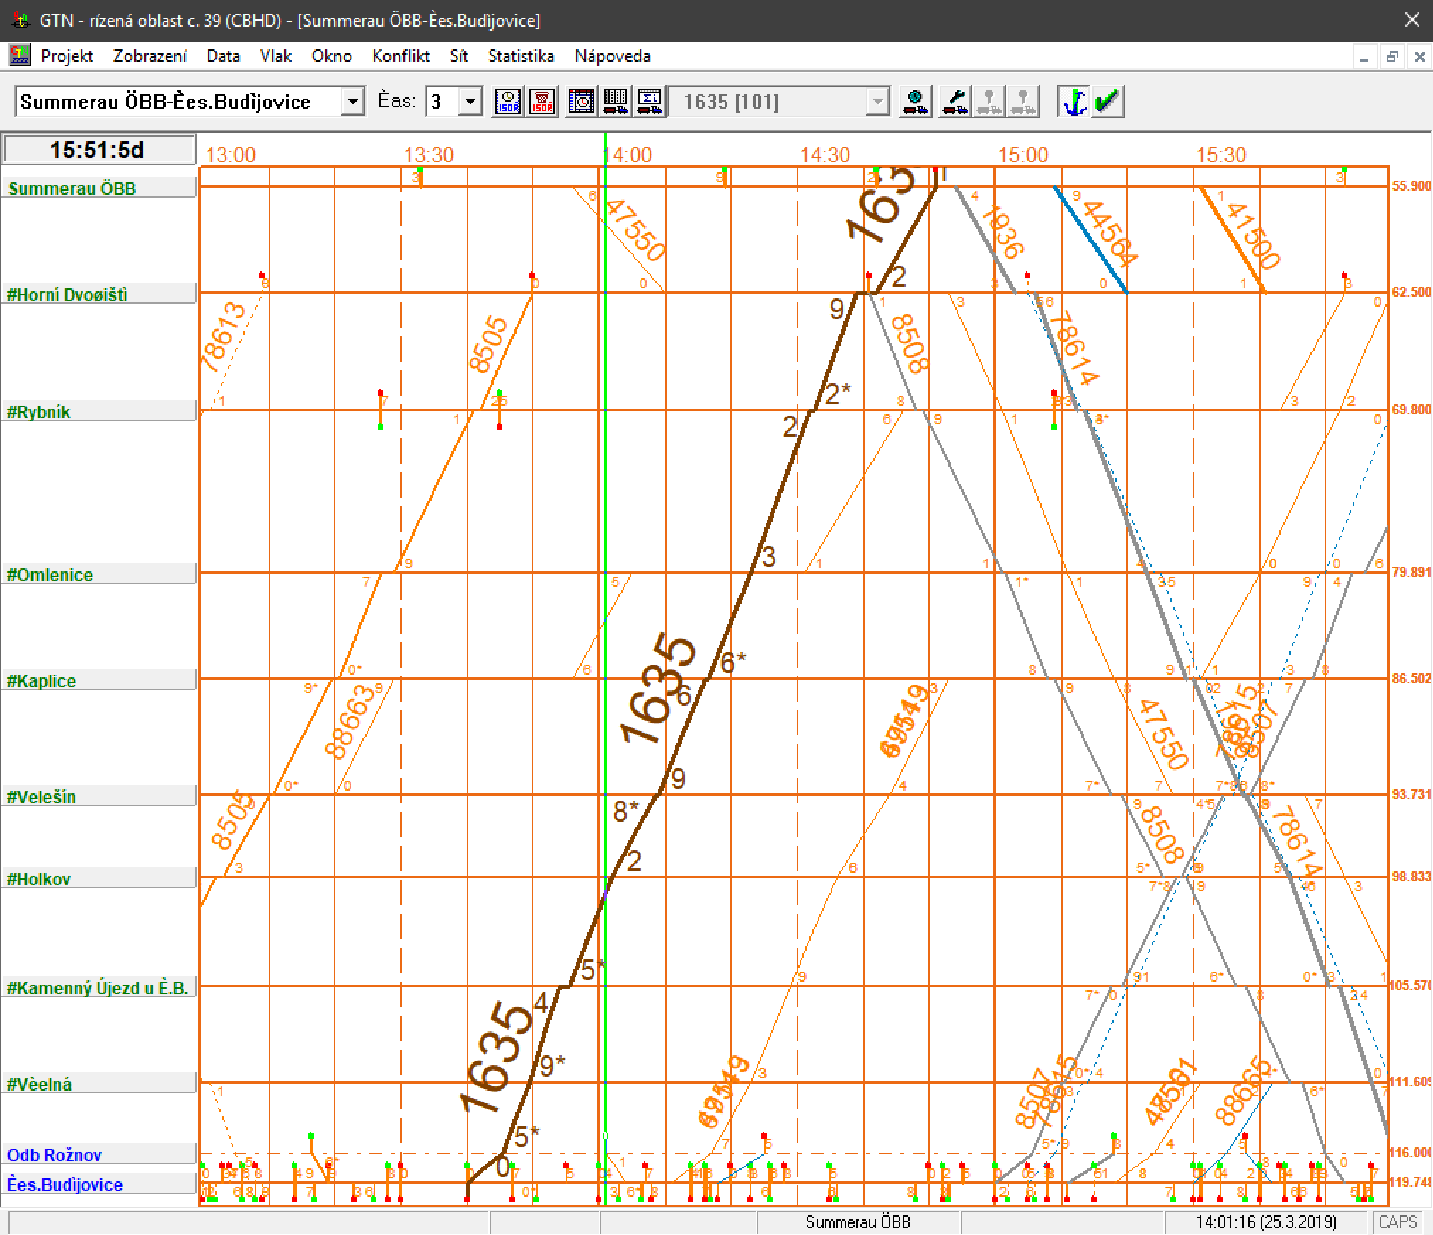
\includegraphics[width=0.75\textwidth]{../img/kap1_gtn_okno_interval_3h}
	\caption{Okno aplikace GTN}
	\label{fig:gtn_okno}
\end{figure}

\subsubsection*{Aplikace v~rámci IS ISOR CDS}
Aplikace pro práci s~grafikonem vlakové dopravy nabízena v~rámci informačního systému ISOR CDS \cite{ISOR_CDS} od OLTIS Group je zaměřena stejně jako aplikace GTN na prohlížení současného provozu. Na obrázku \ref{fig:oltis_window} můžeme vidět, jak aplikace vizualizuje nákresný jízdní řád. Všimněme si, že narozdíl od doposud popisovaného chování nezobrazuje dopravní body na vertikální ose podle jejich kilometrické polohy, ale rozmisťuje je rovnoměrně pro jednodušší zobrazení nákresného jízdního řádu. Taková změna v~zobrazení není nijak závadná, ačkoliv porušuje námi popsané zásady pro zobrazení nákresného jízdního řádu. V dalších částech práce budeme narážet na podobné odchylky, nikdy ale zásadně neporuší popsané rozpoložení uvedené na začátku kapitoly.
Na pravé hraně grafické komponenty zobrazující nákresný jízdní řád nabízí aplikace posuvník pro změnu zobrazené části traťového úseku. Stejným způsobem umožňuje na horizontále výběr zobrazovaného časového intervalu. Obě dvě aplikace tedy nabízí podobné možnosti při zobrazování nákresného jízdního řádu, volí jen jiný způsob ovládání.

\begin{figure}[ht]
	\centering
	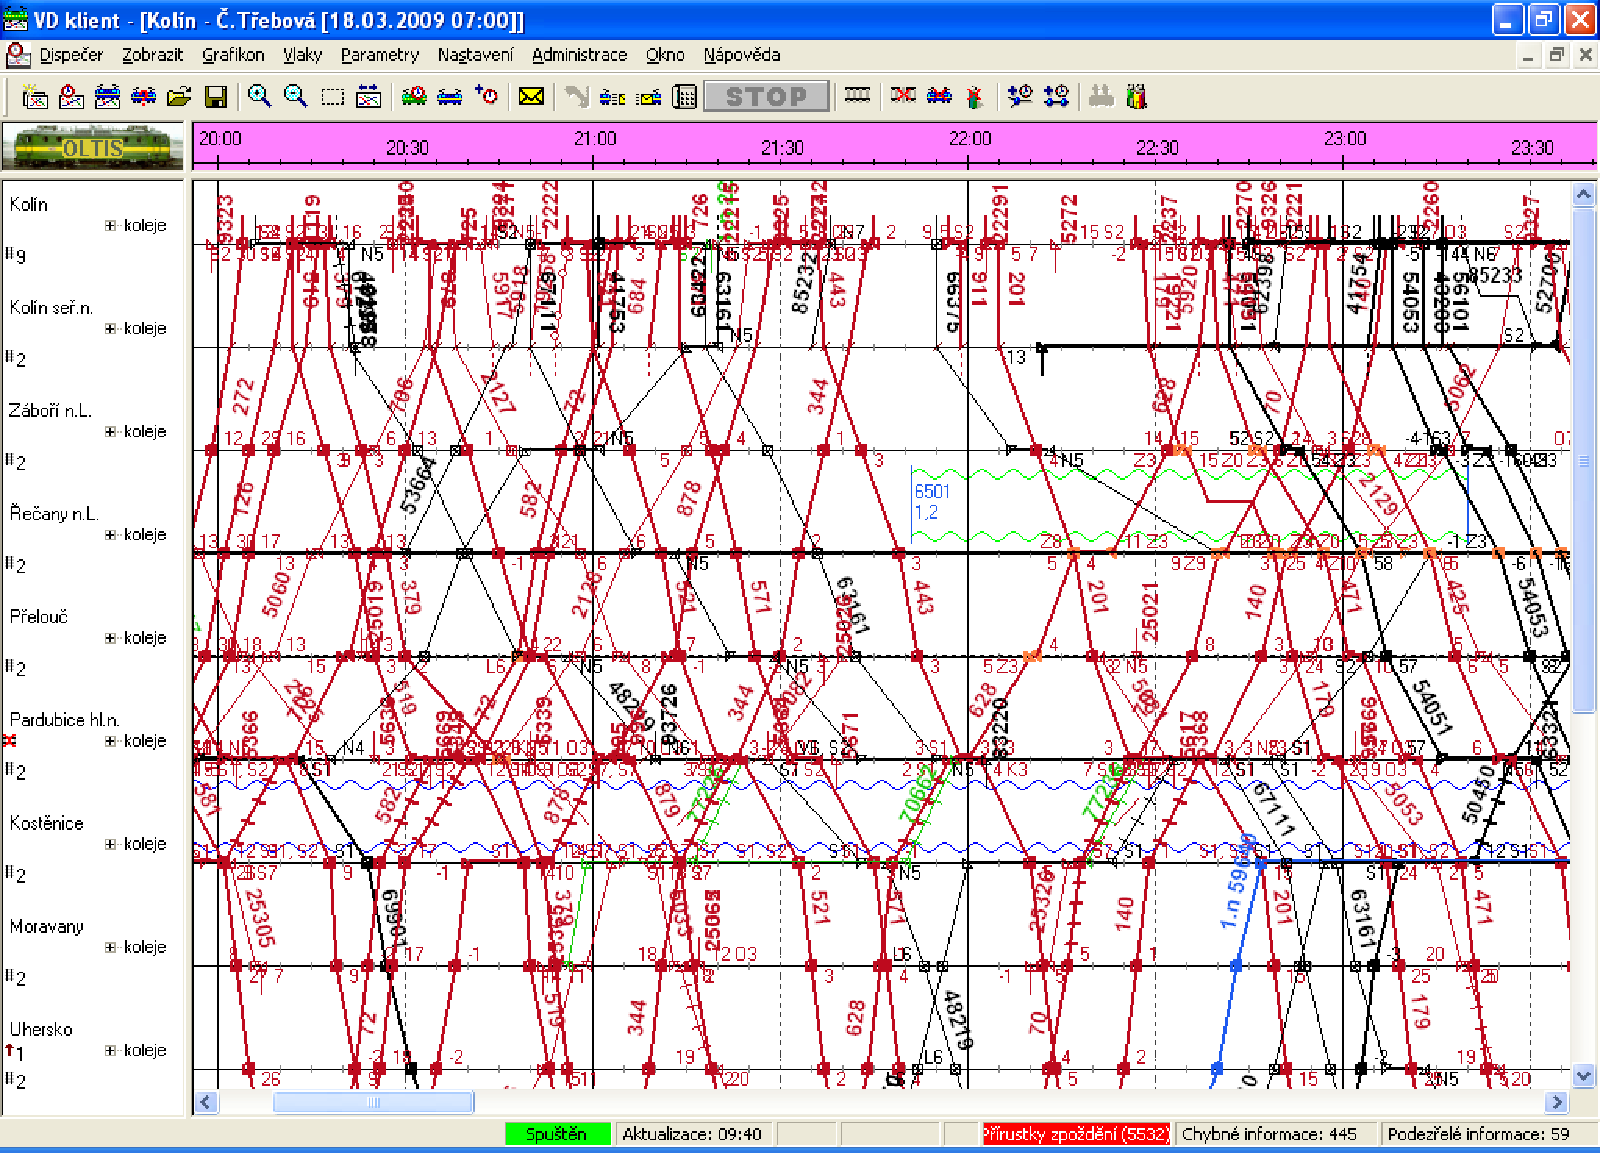
\includegraphics[width=0.9\textwidth]{../img/kap1_ISOR_window}
	\caption{Aplikace Grafikon od OLTIS Group, převzato ze stránky společnosti~\cite{ISOR_CDS}}
	\label{fig:oltis_window}
\end{figure}

\subsection*{Grafikon vlakové dopravy mimo skutečný provoz}
\label{model_gvd}
V~následující části zjistíme, že námi vytvářená grafická komponenta zobrazující nákresný jízdní řád může být součástí aplikací, které nejsou určeny pro nasazení v~reálném provozu. Grafikon vlakové dopravy se zobrazeným nákresným jízdním řádem se nabízí použít i~v~jiných scénářích, zejména pak při aktivitách, které se snaží provoz na železnici simulovat.

\subsubsection{Vytváření studií pro vlakovou dopravu}
Nejblíže problémům vlakové dopravy řešených ve skutečné situaci jsou studie a~koncepty věnující se provozu na železnici, které k~prezentování svých výsledků využívají koncepčně sestavený grafikon vlakové dopravy a~nákresné jízdní řády. Tyto studie jsou většinou zpracovávány v~rámci různých bakalářských a~diplomových prací studentů dopravních fakult. Existují komerční nástroje, které jsou k~těmto účelům určené a~na základě zadaných dat můžou autorům pomoci se sestavením grafikonu vlakové dopravy a~vytvořením jeho pomůcek. Typickým řešením je pro fakultu koupit licenci takového nástroje. Jedním z~těchto nástrojů je FBS-Bahn \cite{FBS_BAHN}. Tímto nástrojem byl vytvořen nákresný jízdní řád na obrázku \ref{fig:studie_njr}.

\begin{figure}[ht]
	\centering
	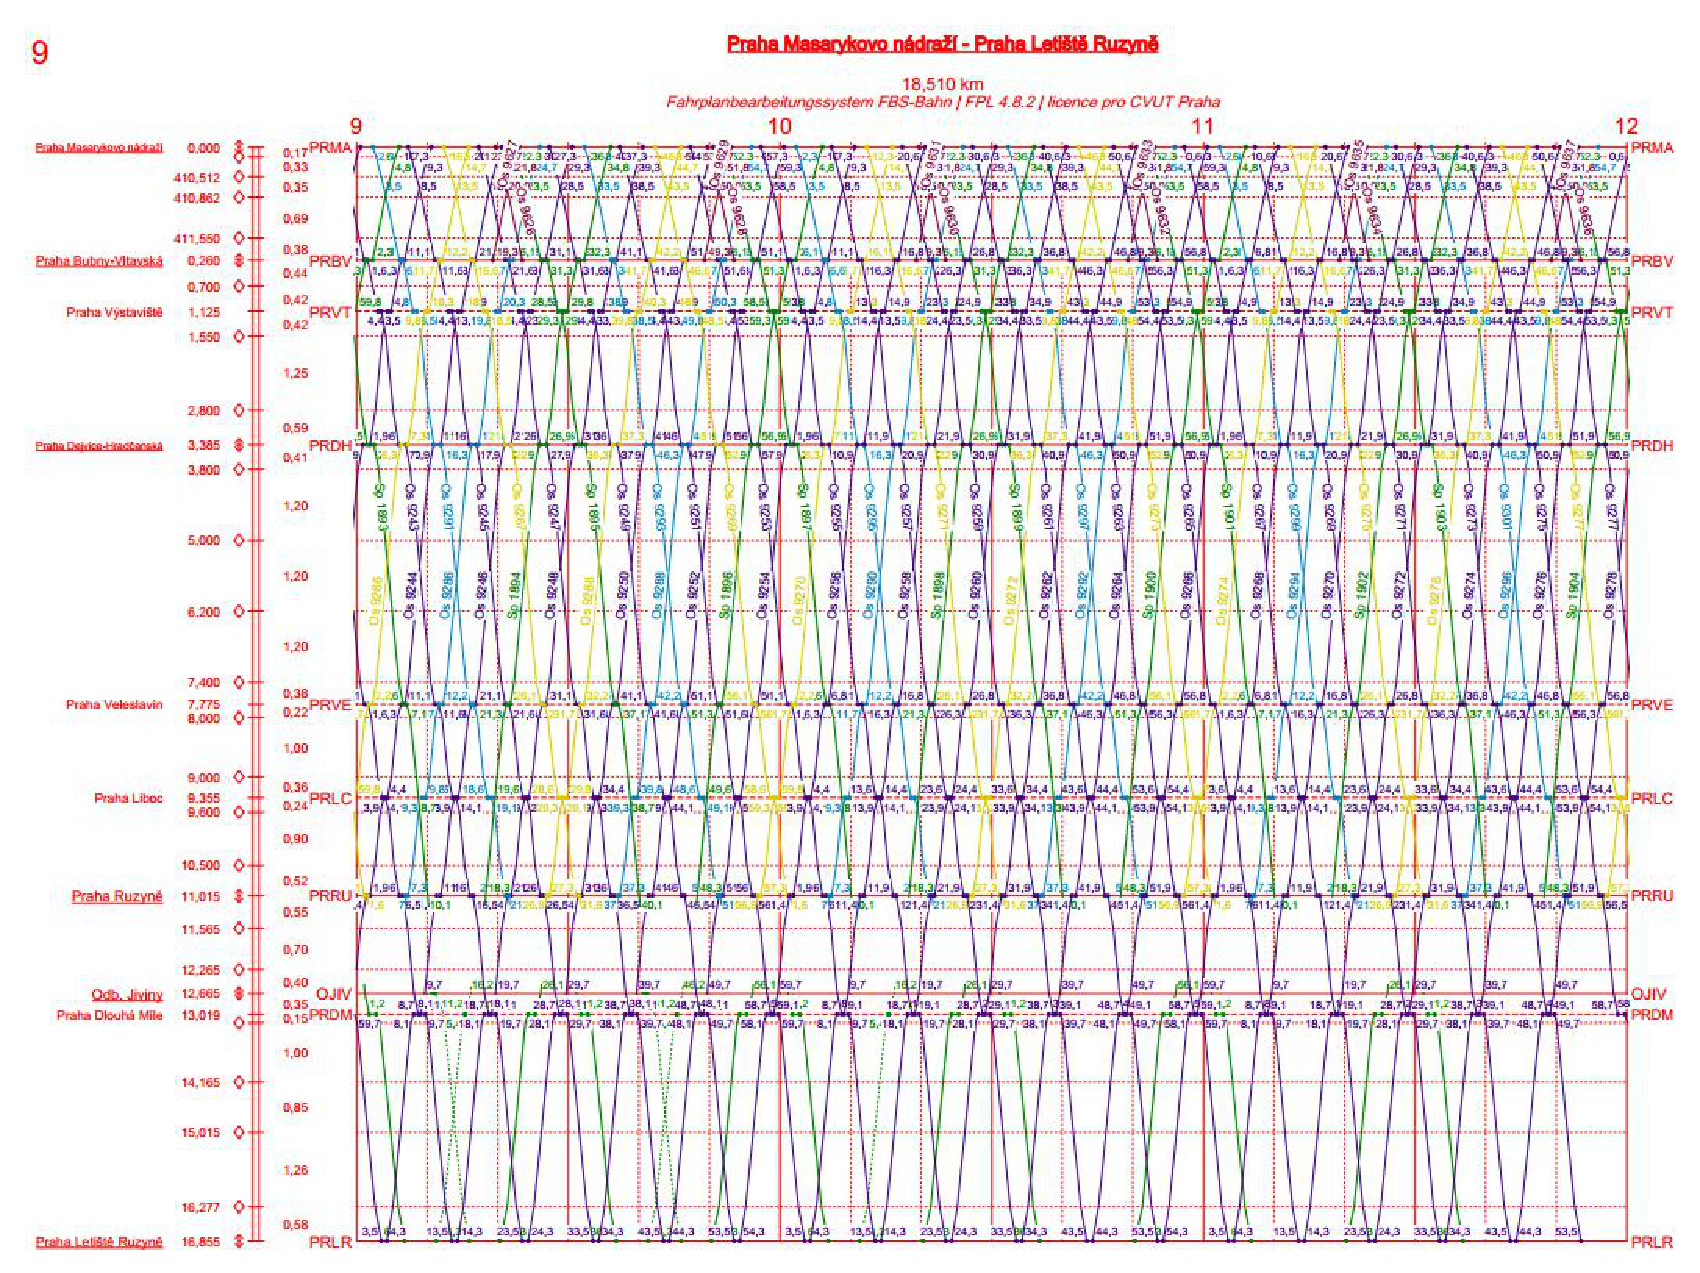
\includegraphics[width=\textwidth]{../img/kap1_studie_njr}
	\caption{Nákresný jízdní řád generovaný nástrojem FBS-Bahn pro diplomovou práci Koncepce obsluhy letiště Ruzyně kolejovou dopravou, M. Drábek~\cite{dipl_drabek}}
	\label{fig:studie_njr}
\end{figure}

\subsubsection{Aplikace v~modelové železnici}
Modelová železnice je co nejvěrnějším ztvárněním skutečné železnice ve zmenšeném měřítku. Za účelem napodobení skutečného provozu se nabízí jízdu vlaků na modelovém kolejišti organizovat podle grafikonu vlakové dopravy. Pokud se řízení vlaků na modelovém kolejišti věnuje více modelářů, v~rámci přípravy jsou jízdy vlaků rozplánovány a~zakresleny do nákresného jízdního řádu, který může být načrtnutý na papír.

Modeláři, kteří umí programovat, můžou vytvářet různé aplikace k~organizaci provozu na modelové železnici. Jednou z~nich je aplikace Grafikon \cite{Grafikon}, zobrazená na obrázku \ref{fig:grafikon_modely}. Aplikace umožňuje sestavit grafikon vlakové dopravy pro modelová kolejiště. Nákresný jízdní řád, který vykresluje, ale slouží pouze k~plánování a~není možné ho při řízení provozu na modelovém kolejišti měnit, třeba pro porovnání současného provozu s~původním plánem. Pro modeláře existují řešení, která umožňují řídit provoz na modelové železnici za pomoci počítače. Výrobci nástrojů pro řízení modelové železnice nabízí rozhraní, vůči kterým je možné vytvářet software sloužící k~sestavení vlakové cesty, kdy modelář může z~počítače měnit třeba nastavení výhybek. Takový software ale zcela nezachycuje proces organizace vlakové dopravy odpovídající skutečné situaci. Vytvářenou grafickou komponentu zobrazující nákresný jízdní řád by pak bylo možné zahrnout do nových nebo stávajících softwarových řešení, kterým by tato komponenta umožnila graficky zaznamenávat jízdy vlaků a~porovnávat je se sestaveným plánem.

\begin{figure}[ht]
	\centering
	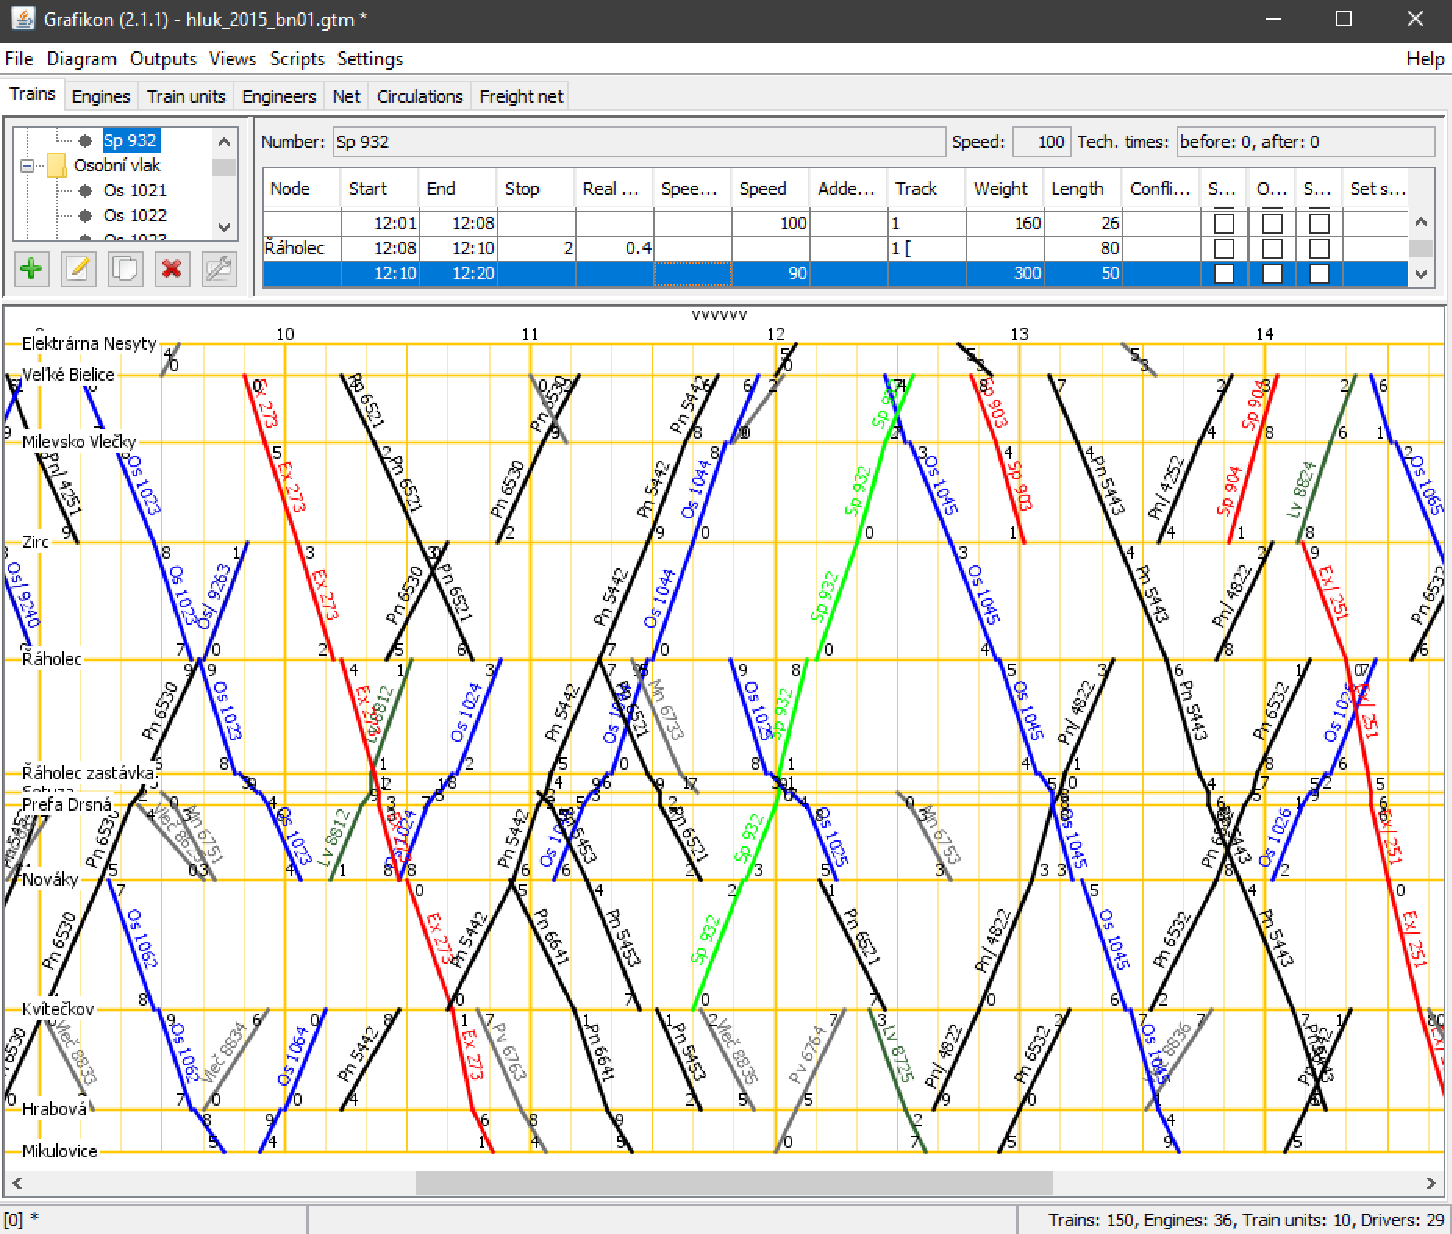
\includegraphics[width=\textwidth]{../img/kap1_grafikon_modely}
	\caption{Hlavní okno aplikace Grafikon určené pro modelové železnice}
	\label{fig:grafikon_modely}
\end{figure}

\subsubsection{Aplikace ve vlakových simulátorech}
\label{uvod:prace_s_grafikony_vlakove_dopravy:simulatory}
Námi vytvářený nástroj může být integrován do počítačových simulátorů, které se věnují řízení vlaku z~pozice strojvůdce. Na začátku tisíciletí vzniklo mnoho takových simulátorů a~her (Trainz \cite{Trainz}, MSTS \cite{MSTS}) vydávaných firmami, bez možnosti přístupu k~jejich zdrojovým kódům. V~posledních letech vznikly open-source projekty snažící se na základě těchto her vytvořit lepší simulátory s~větší konfigurovatelností, jelikož většina původních her už není dále vyvíjena a~podporována. Mezi tyto open-source simulátory patří OpenRails \cite{OpenRails} a~OpenBVE \cite{OpenBVE}. Oba dva tyto simulátory jsou napsané v~jazyce C\#, existují několik let a~jsou stále udržovány.

Simulátory, snažící se napodobit skutečný provoz na trati předpřipraveným scénářem jízd vlaků v~časovém intervalu několika hodin, by bylo užitečné doplnit pomůckami grafikonu vlakové dopravy. Hráči by byla dostupná (třeba v~okně vedle okna simulátoru) aplikace s~grafikonem vlakové dopravy, což v~současnosti ani jeden ze zmíněných open-source projektů nenabízí. Zajímavá by pak byla možnost hrát hru po síti s~dalšími lidmi (což už tyto simulátory umožňují) a~sledovat průběh hraného scénáře v~nákresném jízdním řádu v~porovnání s~původním plánem.

\section[Vývoj aplikací pro práci s~grafikonem vlakové dopravy]{Vývoj aplikací pro práci\\ s~grafikonem vlakové dopravy}

Zaměřme se na proces vývoje aplikací, které budou pracovat s~grafikonem vlakové dopravy. Všimněme si, že pro všechny uvedené příklady aplikací z~podkapitoly \ref{aplikace_gvd} je nezbytné zobrazovat nákresný jízdní řád. Bez komponenty aplikace, která je zodpovědná za jeho vykreslení, by se data z~grafikonu vlakové dopravy stala těžko spojitelnými množinami informací. Kdybychom se rozhodli vytvořit aplikaci pro práci s~grafikonem vlakové dopravy, stáli bychom tak vždy před rozhodnutím, jak tuto komponentu navrhnout. Pokud by existovala knihovna, která poskytne nástroje pro zobrazování nákresného jízdního řádu a~práci s~jeho obsahem, vývoj aplikací pracujících s~grafikonem vlakové dopravy by se tak ulehčil. Proto hlavní část této práce bude věnována vytváření takové knihovny. Námi vytvářenou knihovnu jsme se rozhodli pojmenovat GTTG (Generic Train Traffic Graph\footnote{Název knihovny jsme chtěli co nejvíce přiblížit anglickému názvu pro nákresný jízdní řád, který se lidmi orientující se ve vlakové dopravě většinou označuje jako train graph. Pro případ, že se s~názvem knihovny setká člověk bez představy o~tom, co nákresný jízdní řád je, jsme chtěli vystihnout to, že se nejedná o~graf zobrazující třeba železniční dvojkolí, ale graf zaznamenávající provoz na trati. Proto jsme přidali do názvu slovo traffic. Slovo generic na začátku názvu vystihuje záměr knihovny podporovat práci s~co největším množstvím nákresných jízdních řádů.}).

\subsection*{Knihovna pro platformu .NET}
Knihovnu, která bude představovat grafickou komponentu umožnující práci s~nákresným jízdním řádem, jsme se rozhodli naimplementovat v~jazyce C\#, který je součástí platformy .NET. Odůvodníme si, proč toto rozhodnutí není závadné a~seznámíme se s~knihovnou SkiaSharp \cite{SkiaSharp}, kterou budeme v~naší knihovně používat ke kreslení v~grafické komponentě.

\subsubsection*{Jazyk C\# a~.NET Standard}
Jelikož vytvářená knihovna bude reálně využívána hlavně modeláři, vývojáři nástrojů pro modelové železnice nebo programátory počítačových simulátorů, musí být snadno udržovatelná a~použitelná k~vytváření jejich vlastních implementací nákresného jízdního řádu. Protože knihovna bude většinou součástí nějaké aplikace s~uživatelským rozhraním, je vhodné, aby uživatelům knihovny bylo dostupné množství GUI frameworků, do kterých bude možné knihovnu jako grafickou komponentu zahrnout.

Protože jazyk C\# je jeden z~nejpoužívanějších objektově orientovaných jazyků a~nabízí mnoho GUI frameworků pro tvorbu desktopových aplikací, jeho výběr není v~rozporu s~tímto požadavkem a~můžeme ho použít. Silnou motivací, proč knihovnu implementovat právě v~tomto jazyce, je fakt, že oba dva zmíněné open-source simulátory jsou v~jazyce C\# napsané a~knihovnu tak bude možné v~těchto stávajících projektech využít.

Naší knihovnu bychom zároveň chtěli vytvořit tak, aby byla v~rámci platformy .NET co nejvíce použitelná. Každý spustitelný program, který v~jazyce C\# napíšeme, může být spuštěn pouze vůči některému z~běhových prostředí. Původním běhovým prostředím platformy .NET je .NET Framework, který je určen pro operační systém Windows. Vedle tohoto běhového prostředí existuje Mono, které bylo vytvořeno jako open-source náhražka .NET Frameworku pro operační systémy Linux a~MacOS. V~posledních letech vzniklo běhové prostředí .NET Core, jehož vývoj je řízen společností Microsoft a~je možné ho použít na operačních systémech Windows, Linux a~MacOS. Je v~plánu nahradit .NET Framework a~Mono právě tímto novým běhovým prostředím. Aby bylo možné vytvářet knihovny, které budou použitelné všemi běhovými prostředími, vzniklo rozhraní .NET Standard. Knihovny, které vůči .NET Standard implementujeme, můžou stále používat skoro stejnou část používaných tříd a~implementací, které jsou nabízeny například v~rámci běhového prostředí .NET Framework. Aby .NET Standard docílilo přenositelnosti mezi více běhovými prostředími, určuje rozhraní, které běhová prostředí musí implementovat, aby kód knihovny .NET Standard mohl být na konkrétním běhovém prostředí vykonáván.
Jelikož vytvářená grafická komponenta bude často umístěna v~aplikaci s~GUI frameworkem, který je spustitelný vůči jednomu běhovému prostředí, bude naše knihovna přenositelná v~rámci rozhraní .NET Standard.

\subsubsection*{SkiaSharp}
Naše knihovna potřebuje nějaký nástroj, který bude sloužit k~vykreslování nákresného jízdního řádu. Práce s~tímto nástrojem by měla být lehká, jelikož ho budeme chtít nabídnout uživatelům naší knihovny pro implementaci jejich vlastních typů nákresných jízdních řádů.

Pro jazyk C\# existuje knihovna SkiaSharp, jako wrapper\footnote{Označení pro knihovnu pracující s~cizí funkcionalitou, kterou vhodně upravuje nebo zpřístupňuje uživateli wrapperu, většinou s~žádnými změnami v~sémantice cizí funkcionality, které chce uživatel wrapperu využívat. SkiaSharp jako wrapper překládá volání funkcí z~jazyka C\# do kódu knihovny Skia implementované v~jazyce C++.} nad vysoce výkonnou 2D grafickou knihovnou Skia napsanou v~jazyce C++. Skia nabízí pro uživatele lehké kreslení různých komplexních typů čar a~textu, které nákresné jízdní řády obsahují. Práce s~knihovnou SkiaSharp je lehká, díky její dostupné dokumentaci, zcela nutné pro případ, kdy ji chceme také nabídnout uživatelům naší knihovny.

Knihovna SkiaSharp je navíc přenositelná v~rámci rozhraní .NET Standard, čili je naší knihovnou použitelná a~splňuje i~všechny naše požadavky na grafický nástroj, který bude naše knihovna používat pro vykreslování nákresného jízdního řádu.

\subsection*{Implementace vlastní aplikace}
Abychom mohli předvést využití naší knihovny, rozhodli jsme se vytvořit vzorovou aplikaci pro práci s~grafikonem vlakové dopravy. Aplikace uživatelům umožní prohlížet nákresné jízdní řády vydávané Správou železniční dopravní cesty. Ověříme tak schopnost knihovny podporovat zobrazení specifické implementace nákresného jízdního řádu. Abychom předvedli, jak knihovna podporuje editaci nákresného jízdního řádu, přidáme mód vytvářející náhodnou dopravní situaci na trati, v~rámci které bude možné upravovat interaktivně v~nákresném jízdním řádu jízdy jednotlivých vlaků.

\section{Cíle práce}
\label{kap1:cile_prace}
\begin{enumerate}[label=\color{goalcolor}\textbf{G{\arabic*}}]
	\item \label{uvod:cil:knihovna}Vytvořit knihovnu pro platformu .NET, představující grafickou komponentu, umožňující práci s~nákresnými jízdními řády
	\begin{enumerate}[label=\color{goalcolor}\textbf{\alph*})]
		\item \label{uvod:cil:knihovna:ruzne_typy_njr} Podporovat zobrazování různých typů nákresných jízdních řádů
		\item \label{uvod:cil:knihovna:integrace_do_aplikaci} Podporovat integraci komponenty do aplikací pracujících s~grafikonem vlakové dopravy
		\item \label{uvod:cil:knihovna:replikace_chovani} Umožnit replikovat chování existujících aplikací pracujících s~grafikonem vlakové dopravy
		\item \label{uvod:cil:knihovna:dotnet_standard} Zajistit přenositelnost knihovny na úrovni .NET Standard
	\end{enumerate}

	\item \label{uvod:cil:aplikace} Použít tuto knihovnu pro implementaci aplikace, která bude sloužit pro práci s~grafikonem vlakové dopravy
	\begin{enumerate}[label=\color{goalcolor}\textbf{\alph*})]
		\item \label{uvod:cil:aplikace:staticke_zobrazeni} Aplikace bude interaktivně zobrazovat listy nákresného jízdního řádu vydávané Správou železniční dopravní cesty.
		\item \label{uvod:cil:aplikace:dynamicke_zobrazeni} Aplikace bude pro ilustrační účely knihovny nabízet mód simulující provoz na trati, v~jehož rámci bude možné upravovat výhledovou dopravu.
		\item \label{uvod:cil:aplikace:vice_gui} Aplikace bude navržena tak, aby část pracující s~modelem dat, představující logiku aplikace, byla zapojitelná do více GUI frameworků platformy .NET.
	\end{enumerate}
	
	\item \label{uvod:cil:skia} Ověřit možnost využití 2D grafické knihovny SkiaSharp pro zobrazování komplexních dat obsažených v~nákresných jízdních řádech
\end{enumerate}
